%\documentclass[
  bibliography=totoc,     % Literatur im Inhaltsverzeichnis
  captions=tableheading,  % Tabellenüberschriften
  titlepage=firstiscover, % Titelseite ist Deckblatt
]{scrartcl}

% Paket float verbessern
\usepackage{scrhack}

% Warnung, falls nochmal kompiliert werden muss
\usepackage[aux]{rerunfilecheck}

% unverzichtbare Mathe-Befehle
\usepackage{amsmath}
% viele Mathe-Symbole
\usepackage{amssymb}
% Erweiterungen für amsmath
\usepackage{mathtools}

% Fonteinstellungen
\usepackage{fontspec}
% Latin Modern Fonts werden automatisch geladen
% Alternativ zum Beispiel:
%\setromanfont{Libertinus Serif}
%\setsansfont{Libertinus Sans}
%\setmonofont{Libertinus Mono}

% Wenn man andere Schriftarten gesetzt hat,
% sollte man das Seiten-Layout neu berechnen lassen
\recalctypearea{}

% deutsche Spracheinstellungen
\usepackage[ngerman]{babel}


\usepackage[
  math-style=ISO,    % ┐
  bold-style=ISO,    % │
  sans-style=italic, % │ ISO-Standard folgen
  nabla=upright,     % │
  partial=upright,   % │
  mathrm=sym,        % ┘
  warnings-off={           % ┐
    mathtools-colon,       % │ unnötige Warnungen ausschalten
    mathtools-overbracket, % │
  },                       % ┘
]{unicode-math}

% traditionelle Fonts für Mathematik
\setmathfont{Latin Modern Math}
% Alternativ zum Beispiel:
%\setmathfont{Libertinus Math}

\setmathfont{XITS Math}[range={scr, bfscr}]
\setmathfont{XITS Math}[range={cal, bfcal}, StylisticSet=1]

% Zahlen und Einheiten
\usepackage[
  locale=DE,                   % deutsche Einstellungen
  separate-uncertainty=true,   % immer Unsicherheit mit \pm
  per-mode=symbol-or-fraction, % / in inline math, fraction in display math
]{siunitx}

% chemische Formeln
\usepackage[
  version=4,
  math-greek=default, % ┐ mit unicode-math zusammenarbeiten
  text-greek=default, % ┘
]{mhchem}

% richtige Anführungszeichen
\usepackage[autostyle]{csquotes}

% schöne Brüche im Text
\usepackage{xfrac}

% Standardplatzierung für Floats einstellen
\usepackage{float}
\floatplacement{figure}{htbp}
\floatplacement{table}{htbp}

% Floats innerhalb einer Section halten
\usepackage[
  section, % Floats innerhalb der Section halten
  below,   % unterhalb der Section aber auf der selben Seite ist ok
]{placeins}

% Seite drehen für breite Tabellen: landscape Umgebung
\usepackage{pdflscape}

% Captions schöner machen.
\usepackage[
  labelfont=bf,        % Tabelle x: Abbildung y: ist jetzt fett
  font=small,          % Schrift etwas kleiner als Dokument
  width=0.9\textwidth, % maximale Breite einer Caption schmaler
]{caption}
% subfigure, subtable, subref
\usepackage{subcaption}

% Grafiken können eingebunden werden
\usepackage{graphicx}

% schöne Tabellen
\usepackage{tabularray}
\UseTblrLibrary{booktabs, siunitx}

% Verbesserungen am Schriftbild
\usepackage{microtype}

% Literaturverzeichnis
\usepackage[
  backend=biber,
]{biblatex}
% Quellendatenbank
\addbibresource{lit.bib}
\addbibresource{programme.bib}

% Hyperlinks im Dokument
\usepackage[
  german,
  unicode,        % Unicode in PDF-Attributen erlauben
  pdfusetitle,    % Titel, Autoren und Datum als PDF-Attribute
  pdfcreator={},  % ┐ PDF-Attribute säubern
  pdfproducer={}, % ┘
]{hyperref}
% erweiterte Bookmarks im PDF
\usepackage{bookmark}

% Trennung von Wörtern mit Strichen
\usepackage[shortcuts]{extdash}

\author{%
  Vincent Wirsdörfer\\%
  \href{mailto:vincent.wirsdoerfer@udo.edu}{authorA@udo.edu}%
  \and%
  Joris Daus\\%
  \href{mailto:joris.daus@udo.edu}{authorB@udo.edu}%
}
\publishers{TU Dortmund – Fakultät Physik}


%\begin{document}
\section{Versuchsaufbau und Versuchsdurchführung}
\label{sec:Durchfuehrung}

Es sollen verschiedene Anwendungsbeispiele der Ultraschalltechnik untersucht und erprobt werden.
Dazu gehören unter anderem die Tiefenmessung, die medizinische Diagnostik und die zeitliche Auflösung.
Für die Tiefenmessung wird ein Acrylblock mit Löchern von zwei Seiten vermessen. Die medizinische 
Diagnostik bezieht sich auf die Erkennung von Brustkrebs anhand eines Brustmodells. Die zeitliche 
Auflösung wird mithilfe eines Herzmodells ermittelt, wobei das Herzzeitvolumen bestimmt werden kann.

\subsection{Abstandsmessung mithilfe von Ultraschalltechnik}
Es kann mithilfe von Ultraschalltechnik der Abstand zu einem Objekt in guter Näherung bestimmt werden. 
Dies beruht auf der Laufzeitmessung des Ultraschalls und wird sich nun zunutze gemacht. Über die 
Schallgeschwindigkeit kann der Abstand allein mit der Laufzeit bestimmt werden. So muss nur die 
Laufzeit gemessen werden. Erprobt wird diese Methode anhand eines Acrylblocks mit elf Löchern. Diese 
sind folgendermaßen im Acryblock angeordnet.

\begin{figure}[H]
    \centering
    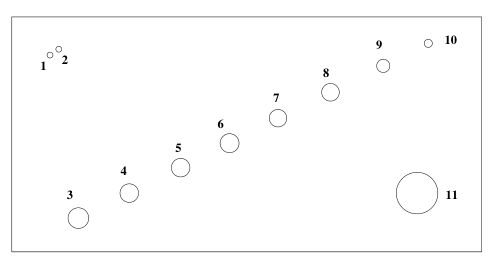
\includegraphics[width=0.6\textwidth]{content/Acrylblock.png}
    \caption{Skizze des Acrylblocks.}
    \label{fig:Acryblock}
\end{figure}

\noindent Die Ultraschallsonde wird zunächst auf die obere Kante mit Kontaktmittel gelegt. Von dort wird mithilfe 
des A-Scans die Laufzeit zu jedem Loch gemessen. Dabei ist zu erwähnen, dass es sich um die Laufzeit 
des Hin- und Rückwegs handelt, weshalb dementsprechend die zweifache Strecke gemessen wird. Die Löcher werden 
chronologisch vermessen. Nach der Messung des letzten Lochs Nr.11, wird der Acrylblock umgedreht 
und die Ultraschallsonde mit Kontaktmittel auf die Unterseite gestellt. Die Unterseite ist also durch 
die Drehung nun oben. Alle Löcher werden wie vorher der Reiche nach mit dem A-Scan vermessen. \\

\noindent Um Referenzwerte für die Durchmesser der Löcher zu bekommen, werden die gemessenen Strecken 
mit dem Messschieber ausgemessen. Es wird also analog die Dicke des Acryls zwischen Loch und Ober- 
beziehungsweise Unterkante vermessen. Damit der Lochdurchmesser bestimmt werden kann, wird die 
Gesamthöhe des Acrylblocks ebenfalls bestimmt. 


\subsection{Medizinische Diagnostik - Tumorerkennung}
Die Ultraschalltechnik ist in der Medizin weit verbreitet und wird als bildgebendes Verfahren häufig 
verwendet. Dies wird am Beispiel von Brustkrebs erprobt. Untersucht wird ein Brustmodell aus Silikon 
mit zwei Tumoren. Zunächst muss der Brustkrebs lokalisiert werden, wofür das Modell abgetastet wird. 
Es können per Hand zwei Tumore festgestellt werden. Diese befinden sich oberhalb und rechts neben 
der Brustwarze und werden in der folgenden Abbildung umkreist. 

\begin{figure}[H]
    \centering
    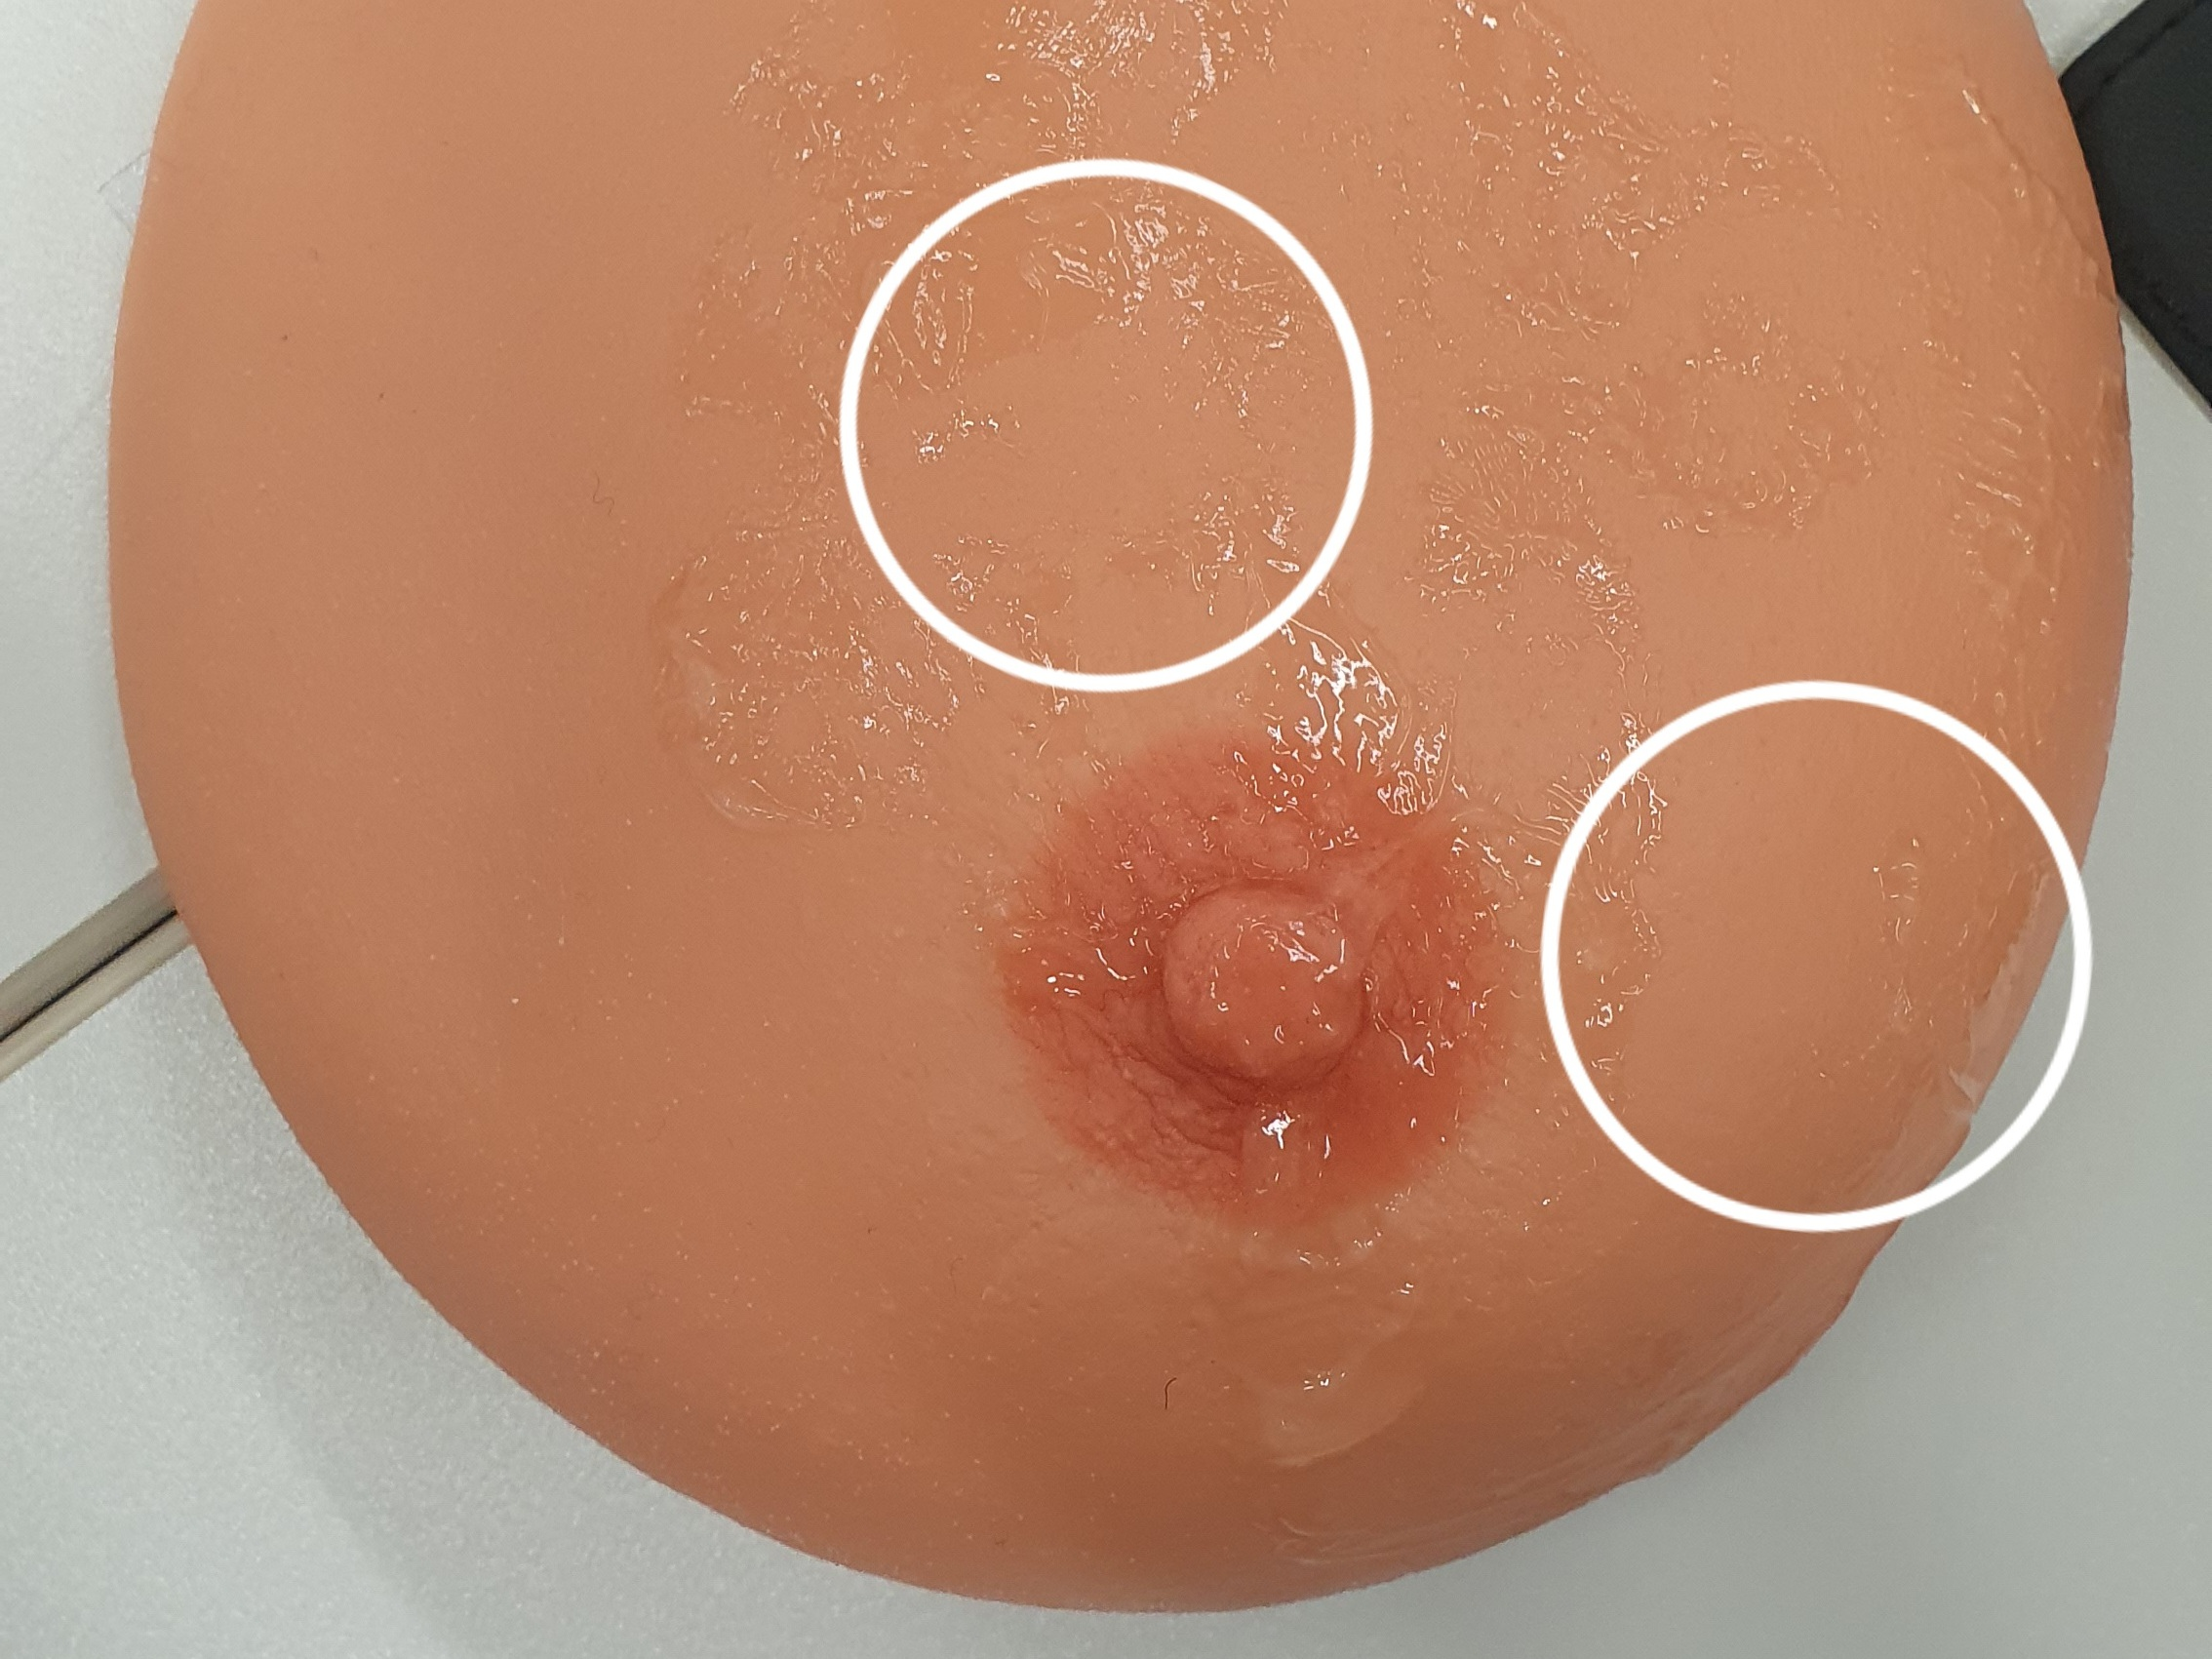
\includegraphics[width = 0.8\textwidth]{content/Tumororientierung2.jpg}
    \caption{Lokalisierung der Tumoren am Modell \cite{Versuchsanleitung_US2}.}
    \label{fig:Acrylblock}
\end{figure}
 
\noindent Diese beiden Tumore werden nun mithilfe des B-Scans visualisiert. Es wird dafür mit der 
Ultraschallsonde ein Schnittbild der Brust aufgenommen, auf dem der Tumor zu erkennen ist. Zwischen 
Ultraschallkopf und Silikon wird Ultraschallgel als Kontakt- und Gleitmittel aufgetragen. Die Sonde 
muss mit konstanter Geschwindigkeit in einer Linie über den Tumor gefahren werden. Anschließend wird 
die verstrichene Strecke mit dem Messschieber vermessen und in das Programm eingetragen. Die Skala 
auf dem Scan wird so in eine Strecke umgewandelt, damit die Größe des Tumors ausgewertet werden kann.
Die Cursors in dem Computerprogramm werden um den Tumor herum gelegt, sodass die Ausdehnung direkt 
berechnet wird. Im Anschluss werden die Scan-Bilder abgespeichert. 


\newpage
\subsection{Vermessung des Auges}
Mithilfe der Abstandsmessung kann auch ein menschliches Augenmodell vermessen werden.
\begin{wrapfigure}{H}{0.3\textwidth}
   % \vspace{-20pt}
    \begin{center}
        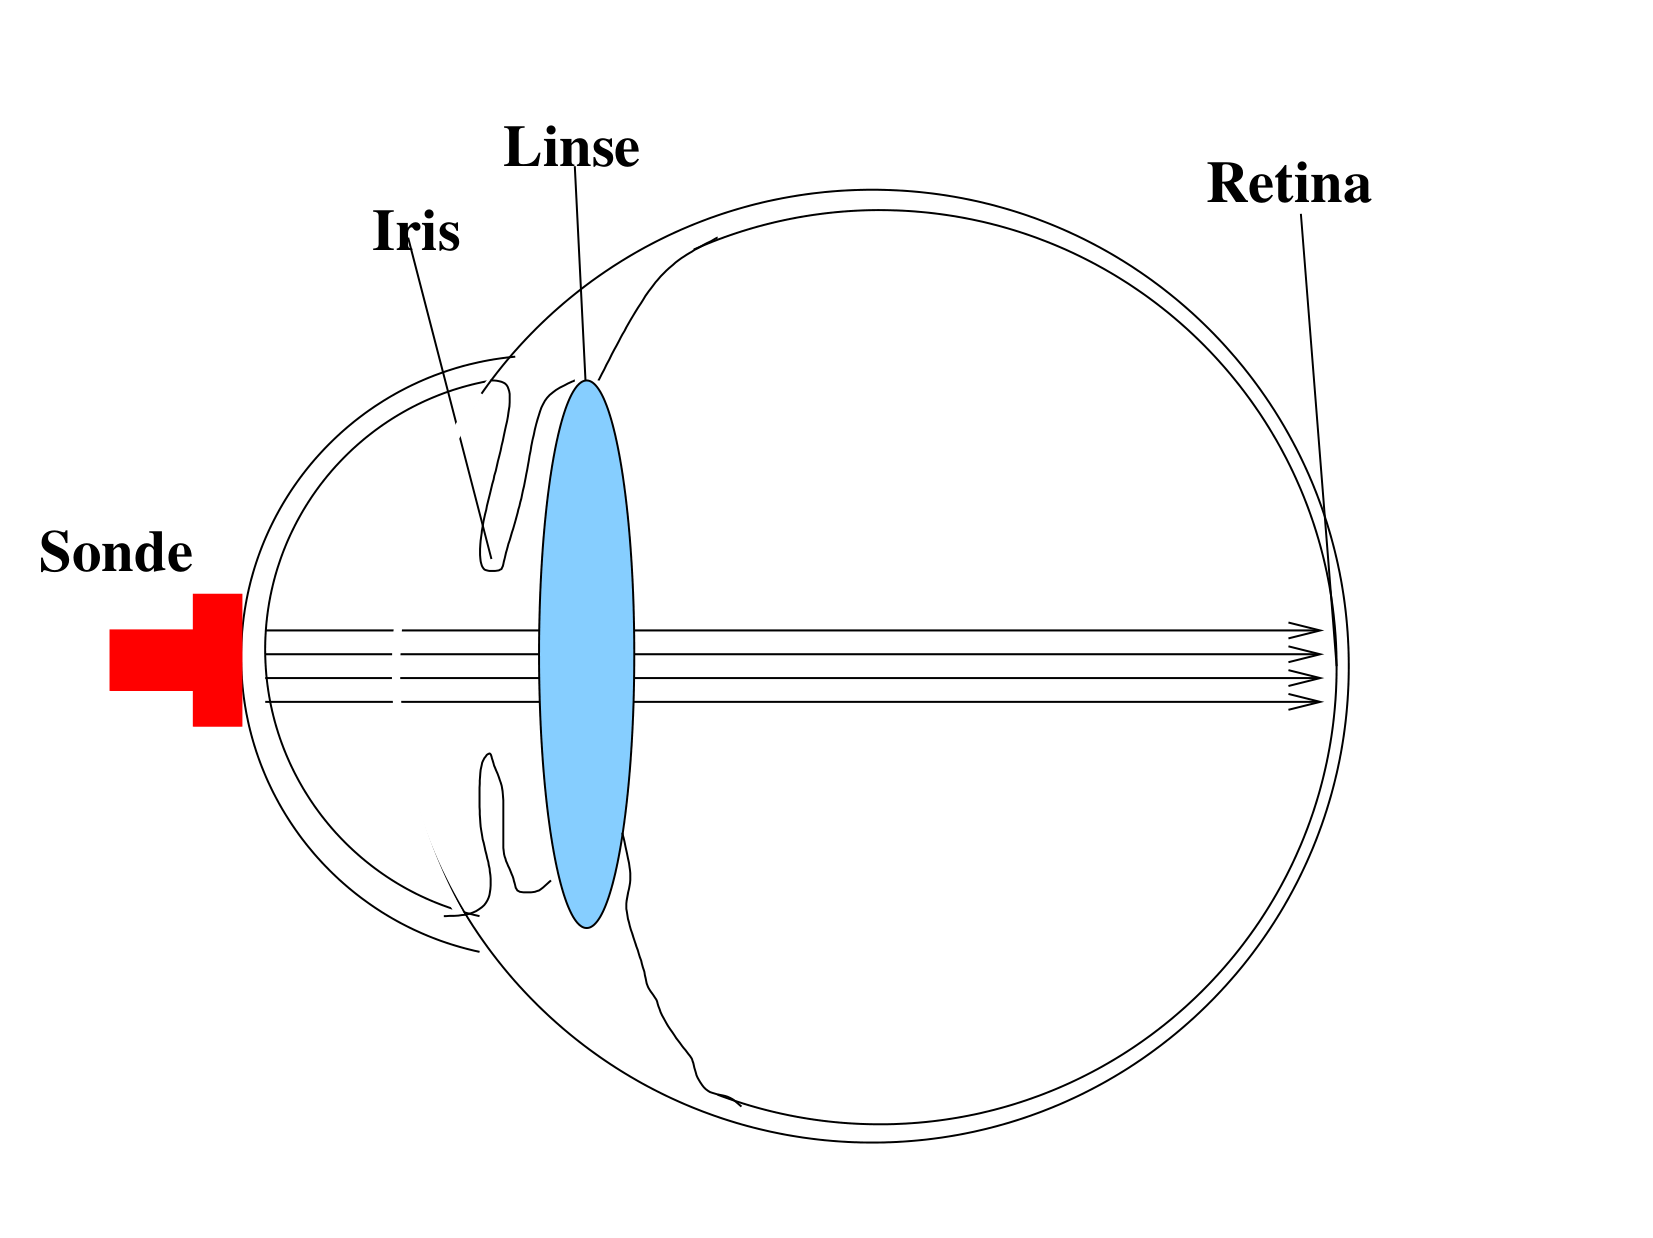
\includegraphics[height=3cm]{content/Augenmodell.png}
        \caption{Skizze des Augenmodells \cite{Versuchsanleitung_US2}.}
    \end{center}
    \label{fig:Augenmodell}
\end{wrapfigure}
Das Augenmodell aus der nachfolgenden Graphik besitzt eine Iris, eine Linse und eine Retina, 
welche mithilfe des Ultraschalls lokalisiert werden sollen.
Dazu wird auf die Modellhornhaut etwas Ultraschallgel als Kontaktmittel 
gegeben und die Ultraschallsonde aufgesetzt. Mit leichtem Druck wird die Rundung der Hornhaut 
verringert, sodass die Sonde einen guten Kontakt zum Modell hat. Auf dem Computer wird der A-Scan 
eingestellt. Die Sonde wird mit der Hand feinfühlig so ausgerichtet, dass mehrere Peaks im A-Scan 
zusehen sind. Wenn dies der Fall ist, wird der Scann eingefroren, sodass er ausgewertet werden kann.
Da im Auge verschiedene Teile vorhanden sind, wird der Schall an unterschiedlichen Stellen 
reflektiert und durchläuft verschiedene Bereiche mit unterschiedlichen Medien. An den Grenzschichten 
der Medien wird er reflektiert, was dann als Peak im Computerprogramm zusehen ist. 


\subsection{Herzzeitvolumen}

Um das Herzzeitvolumen zu bestimmen, wird die zeitliche Auflösung der Ultraschalltechnik verwendet. 
Es wird dazu erneut ein B-Scan angefertigt. Die Sonde bleibt jedoch stationär und der zu scannende 
Bereich verändert sich. Zur Durchführung wird ein Zylinder mit Wasser gefüllt. Der Ultraschallkopf 
muss stabil auf der Wasseroberfläche per Hand gehalten werden. Am Boden dieses 
Zylinders ist ein Gummi angebracht. Dieses Gummi ist mit einer Luftpumpe verbunden, sodass per Hand 
Luft in und aus dem Gummi gepumpt wird. Dadurch dehnt sich das Gummi aus und der Boden des Zylinders 
hebt und senkt sich. Der B-Scan erfasst diese Hebungen und Senkungen. Weil der B-Scan zeitlich 
begrenzt ist, können nur beschränkt viele Zyklen erfasst werden. Es wird eine geeignete Pumpfrequenz 
gewählt, mit welcher das Gummi aufgeblasen wird, sodass zehn Zyklen vom B-Scan erfasst werden. Auf 
dem B-Scan sind nun Ausschläge zu erkennen. Mit den Cursorn werden die Dauer des Pumpens und die Höhe, um 
die sich das Gummi erhebt, vermessen. Der B-Scan wird anschließend als Graphik gespeichert.


%\section{Versuchsdurchführung}

%\section{Messwerte}

%\end{document}

